\subsection{Recurrent neural networks}
\label{sec:recurrent_neural_networks}

The problem with the feedforward language model is that it has a fixed window size.
We can use a \textbf{recurrent neural network} to solve this problem.

The idea is to summarize every new word the model sees in a \textbf{hidden state}.
Then the model will use this hidden state to predict the next word.
\[
    P[w_{i+1}|w_1,\dots,w_i]=P[w_{i+1}|h_i]
\]
Where $h_i$ is the hidden state of the model up to position $i$.

The hidden state is computed as:
\[
    h_i=f(e_i,h_{i-1})
\]
($e_i$ is the embedding of the word $w_i$).

In this context we usually speak about time step $t$ instead of position $i$.

\begin{figure}[H]
    \centering
    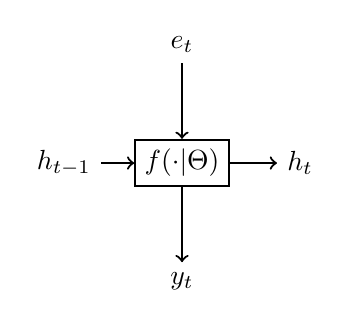
\begin{tikzpicture}[node distance=1.5cm, auto, thick]
        % Nodes
        \node (f) [draw, rectangle] {$f(\cdot|\Theta)$};
        \node (h_old) [left of=f] {$h_{t-1}$};
        \node (e) [above of=f] {$e_t$};
        \node (h) [right of=f] {$h_t$};
        \node (y) [below of=f] {$y_t$};

        % Edges
        \draw[->] (h_old) -- (f);
        \draw[->] (e) -- (f);
        \draw[->] (f) -- (h);
        \draw[->] (f) -- (y);
    \end{tikzpicture}
    \caption{RNN cell}
    \label{fig:rnn_cell}
\end{figure}

The RNN is a parametrized learnable function $f(\cdot|\Theta)$ s.t.
\[
    f(e_t,h_{t-1}|\Theta): \mathbb{R}^{1\times d}\times\mathbb{R}^{1\times h}\rightarrow\mathbb{R}^{1\times h}\times\mathbb{R}^{1\times m}
\]

$f$ is called the \textbf{RNN cell}.

Given a RNN cell, a sequence of $n$ words $w_1,\dots,w_n$ and their embeddings $e_1,\dots,e_n$ and $h_0=0$
we can compute the hidden states and the output of the model as follows:
\[
    h_t,y_t=f(e_t,h_{t-1}|\Theta)
\]

\begin{figure}[H]
    \centering
    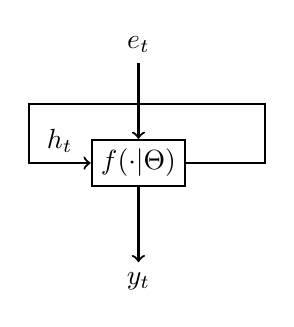
\begin{tikzpicture}[node distance=1.5cm, auto, thick]
        % Nodes
        \node (f) [draw, rectangle] {$f(\cdot|\Theta)$};
        \node (e) [above of=f] {$e_t$};
        \node (y) [below of=f] {$y_t$};

        % Edges
        \draw[->] (e) -- (f);
        \draw[->] (f) -- (y);
        \draw[->] (f.east) -- +(1,0) -- +(1,0.75) -- +(-2,0.75) -- +(-2,0) -- (f.west) node[above, pos=0.5] {$h_t$};
    \end{tikzpicture}
    \caption{RNN model}
    \label{fig:rnn_model}
\end{figure}


